% !TeX spellcheck = en_US	


\documentclass[10pt,journal,compsoc]{IEEEtran}
\usepackage{graphicx}
\usepackage[ruled, noend]{algorithm2e}
\usepackage{url}
\usepackage{epstopdf}
\usepackage{indentfirst}
\usepackage[tight,footnotesize]{subfigure}
\usepackage{amsmath}
\usepackage{amssymb}
\usepackage{multirow}
\usepackage{color}
\usepackage{enumerate}

\newtheorem{Formula}{Formula}
\newtheorem{Lemma}{Lemma}
\newtheorem{Corollary}{Corollary}
\newtheorem{Property}{Property}
\newtheorem{Rule}{Rule}

% *** CITATION PACKAGES ***
\ifCLASSOPTIONcompsoc
\usepackage[nocompress]{cite}
\else
\usepackage{cite}
\fi


\begin{document}


\title{Checking Big Suffix and LCP Arrays by Probabilistic Methods}

\author{
	Yi~Wu,
	Ge~Nong,
	Wai~Hong~Chan,
	Ling~Bo~Han% <-this % stops a space
	\IEEEcompsocitemizethanks{
		\IEEEcompsocthanksitem Y. Wu, G. Nong (corresponding author) and L.~B.~Han are with the Department of Computer Science, Sun Yat-sen University, Guangzhou 510275, China. E-mails: wu.yi.christian@gmail.com, issng@mail.sysu.edu.cn, hanlb@mail2.sysu.edu.cn.
		
		\IEEEcompsocthanksitem Wai Hong Chan (corresponding author) is with the Department of Mathematics and Information Technology, The Education University of Hong Kong, Hong Kong. E-mail: waihchan@ied.edu.hk.
}}% <-this % stops a space
	
\IEEEtitleabstractindextext{%
\begin{abstract}

	For full-text indexing of massive data, the suffix and LCP (longest common prefix) arrays have been recognized as the fundamental data structures and should be verified to ensure their correctness after construction. We propose in this paper two methods to probablisitically check the suffix and LCP arrays in external memory by using a Karp-Rabin fingerprinting function, in terms of that the checking result is wrong with only a negligible probability. The first method checks the lexical order and the LCP-value of two neighboring suffixes in the given suffix array by computing and comparing the fingerprints of their LCPs. The second method first applies the fingerprinting technique to check a subset of the given suffix and LCP arrays, then it produces the whole arrays from the verified parts following the induced-sorting principle and compares the induced and input copies with each other for verification.
	
	
\end{abstract}

% Note that keywords are not normally used for peerreview papers.
\begin{IEEEkeywords}
	Suffix and LCP arrays, verification, Karp-Rabin fingerprinting function.
\end{IEEEkeywords}}


% make the title area
\maketitle

\IEEEdisplaynontitleabstractindextext

\IEEEpeerreviewmaketitle

\section{Introduction}\label{sec:introduction}

\subsection{Background} \label{sec:introduction:background}


Suffix and longest common prefix (LCP) arrays play an important role in various string processing tasks, such as data compression, pattern matching and genome assembly. In dozens of applications, these two data structures are combined to constitute a powerful full-text index for massive data, called enhanced suffix array~\cite{Abouelhodaa2004}, which is more space efficient than suffix tree and applicable to emulating any searching functionalities provided by the latter in the same time complexity. During the past decades, much effort has been put on the development of designing efficient suffix array construction algorithms~(SACAs). Specifically, the first internal-memory algorithm for building SA was introduced in~\cite{Manber1993}. From then on, a plethora of SACAs have been proposed on different computation models, e.g., internal memory~\cite{Karkkainen2003, Ko2003, Kim2003, Nong11}, external memory~\cite{Dementiev2008, Ferragina2012, Manzini2004, Bingmann12, Karkkainen2014, Nong14, Nong15} and shared memory models~\cite{Osipov2012, Deo2013, Wang2015, Karkkainen2015}. In respect of the design on LCP-array construction algorithms~(LACAs), the existing works can be classified into two categories, where the algorithms of the first category compute the suffix and LCP arrays in the same time~\cite{Fischer11, Bingmann12, Flick2015} and that of the second category take the suffix array (SA) and/or Burrows-Wheeler transform (BWT) as input to facilitate the computation~\cite{Kasai2001,Karkkainen2009, Fischer11, Puglisi2008, Puglisi2008, Deo2013, Karkkainen2016}.


While the study for efficient construction of suffix and LCP arrays is evolving, the programs implementing the proposed algorithms are commonly provided ``as is", with the purpose only for the performance evaluation experiemnts of the articles where they are reported. That is, these programms give no guarantee that they have correctly implemented the proposed algorithms. The programs for recently proprosed algorithms are becoming much more complicated than before, casuing more difficulties for program verifying and debugging\footnote{In our studies before, we have exprienced problems caused by bugs of the exisitng programs.}. As a common practice, a suffix or LCP array checker is also provided for verifying the correctness of a constructed array. For example, such a checker is provided in the software packages eSAIS \cite{xxx} (DC3, pScan and etc? more and better) for constructing suffix and/or LCP arrays. In addition to help avoid implementation bugs, a checker is also demanded for an array constructed by a probabilistic algorithm \cite{xxx}. In this case, the array is correct with a probability and hence must be verified by a checker to ensure its correctness.

As far as we know, the work presented in~\cite{Burkhardt2003} is the only SA checking method that can be found in the existing literature, and no efficient approach for the LCP-array verification has been reported yet. In particular, there is currently no reported solution that can check both the suffix and the LCP arrays in external memory. This motivates our work here to design efficient external memory algorithms for checking the suffix and LCP arrays of massive data.
	
\subsection{Contribution}\label{sec:introduction:contribution}

Our contribution includes two checking methods for the given suffix and LCP arrays in external memory. 

The main idea of the first method is to test the lexical order and the LCP-value of two neighboring suffixes in a suffix array by literally comparing their characters. To reduce time complexity for a comparison between two sequences of characters, a Karp-Rabin fingerprinting function is employed to transform each sequence into a single integer, called fingerprint, such that the equality of two sequences can be correctly checked with a negiligible error probability by comparing their fingerprints in constant time. 

By using the same fingerprinting technique, the second method first verifies a subset chosen from the input arrays and then produces a copy of the suffix and LCP arrays from the verified subset following the induced sorting principle. Given that the inducing process is correct, the input arrays are considered to be right with a high probability if they are equal to the induced copies. 

The remainder of this paper is organized as follows. We first describe the proposed two checking methods in Sections~\ref{sec:method1} and~\ref{sec:method2}, then present the experimental results in Section~\ref{sec:experiment},and give the conclusion in Section~\ref{sec:conclusion}.


\section{Method A} \label{sec:method1}


\subsection{Preliminaries} \label{sec:method1:notations}

Given an input string $x$ drawn from an alphabet $\Sigma$, we assume that $x[n - 1] = \$$ and $\$ \in \Sigma$ is smaller than any other characters in $x$. The suffix array of $x$, denoted by $sa$, is a permutation of $\{0, 1, ..., n - 1\}$ such that ${\sf suf}(sa[i]) < {\sf suf}(sa[j])$ for all $0 \le i < j < n$, where ${\sf suf}(sa[i])$ and ${\sf suf}(sa[j])$ are the suffixes starting with $x[sa[i]]$ and $x[sa[j]]$, respectively. Particularly, ${\sf suf}(sa[i])$ is a lexical neighbor of ${\sf suf}(sa[j])$ if $|i - j| = 1$. The LCP array of $x$, denoted by $lcp$, consists of $n$ integers, where $lcp[i]$ records the LCP-value of ${\sf suf}(sa[i])$ and its left neighbor in $sa$ for $i \in [1, n)$. 


\subsection{Idea} \label{sec:method1:idea}

The lexical order and the LCP-value of ${\sf suf}(sa[i])$ and ${\sf suf}(sa[j])$ can be determined by literally comparing their characters from left to right. Because all the suffixes differ in length and end with a common character, there must exist $k \in [0, n)$ such that $x[i, i + k) = x[j, j + k)$ and $x[i + k] \ne x[j + k]$. According to Lemma~\ref{lemma:1}, this method can be also applied to checking suffix and LCP arrays, but it suffers from high time complexity as the two substrings indicated by the LCP-value for each pair of neighboring suffixes in $sa$ take at most $\mathcal{O}(n)$ character-wise comparisons.

\begin{Lemma} \label{lemma:1}
	Both $sa[0, n)$ and $lcp[0, n)$ are correct if and only if the following conditions are satisfied, for all $i \in [1, n)$:
	\begin{enumerate}[(1)]
		\item
		$sa$ is a permutation of $\{0, 1, \dots, n - 1\}$.
		\item
		$x[sa[i], sa[i] + lcp[i] - 1] = x[sa[i - 1], sa[i - 1] + lcp[i] - 1]$.
		\item
		$x[sa[i] + lcp[i]] > x[sa[i - 1] + lcp[i]]$. 	
	\end{enumerate}
\end{Lemma}

\begin{IEEEproof}
	Both the sufficiency and necessity are immediately seen from the definition of suffix and LCP arrays. Specifically, condition (1) demonstrates that all the suffixes in $x$ are sorted in $sa$, while conditions (2)-(3) indicate that the lexical order and the LCP-value of any two neighboring suffixes in $sa$ are both correct.
\end{IEEEproof}

An alternative is to exploit a perfect hash function~(PHF) to convert each substring into a single integer such that any two substrings have a common hash value if and only if they are literally equal to each other. Hence, the equality of two substrings can be determined by comparing the corresponding hash values instead. The key point here is how to efficiently compute the hash values of $x[sa[i], sa[i] + lcp[i] - 1]$ and $x[sa[i - 1], sa[i - 1] + lcp[i] - 1]$ for all $i \in [1, n)$. Taking into account the high cost of finding a PHF to meet this requirement, we prefer using a Karp-Rabin fingerprinting function~\cite{Karp1987} to transform a substring into its integer form, called fingerprint. Specifically, suppose $L$ is a prime and $\delta$ is randomly chosen from $[1, L)$, the fingerprint ${\sf fp}(i, j)$ of a substring $x[i, j]$ can be calculated according to the formulas listed below: scan $x$ rightward and use Formulas~\ref{formula:1}-\ref{formula:2} to iteratively compute ${\sf fp}(0, k)$ for all $k \in [0, n)$, record ${\sf fp}(0, i - 1)$ and ${\sf fp}(0, j)$ during the scan and subtract the former from the latter to obtain ${\sf fp}(i, j)$ following Formula~\ref{formula:3}. 

\begin{Formula} \label{formula:1}
	${\sf fp}(0, -1) = 0$.
	
\end{Formula}

\begin{Formula} \label{formula:2}	
	${\sf fp}(0, i) = {\sf fp}(0, i - 1) \cdot {\delta} + x[i]\mod L$ for $i \ge 0$.
	
\end{Formula}

\begin{Formula} \label{formula:3}
	${\sf fp}(i, j) = {\sf fp}(0, j) - {\sf fp}(0 ,i - 1) \cdot {\delta}^{j - i + 1}\mod L$.
	
\end{Formula}

It is worthy of pointing out that two equal substrings always share a common fingerprint, but the inverse is not true. Fortunately, it has been proved in~\cite{Karp1987} that the probability of a false match can be reduced to a negligible level by setting $L$ to a large value\footnote{This property is utilized in~\cite{Bille2013} to design a probabilistic algorithm for computing a sparse suffix array. }. This leads us to the following conclusion.

\begin{Corollary} \label{corollary:1}
	Both $sa[0, n)$ and $lcp[0, n)$ are correct with a high probability given the following conditions, for all $i \in [1, n)$:
	
	\begin{enumerate}[(1)]
		\item
		$sa$ is a permutation of $\{0, 1, \dots, n - 1\}$.
		
		\item
		${\sf fp}(sa[i], sa[i] + lcp[i] - 1) = {\sf fp}(sa[i - 1], sa[i - 1] + lcp[i] - 1)$.
		
		\item
		$x[sa[i] + lcp[i]] > x[sa[i - 1] + lcp[i]]$.
	\end{enumerate}
\end{Corollary}

In the rest of this section, we describe the algorithm for checking the given suffix and LCP arrays using external memory based on this conclusion. 

\subsection{Algorithm} \label{sec:method1:algorithm}

Following the discussion in Section~\ref{sec:method1:idea}, the conditions of Corollary~\ref{corollary:1} can be checked using $\mathcal{O}(n)$ time and space in random access models by the 2-step procedure below:

\begin{itemize}
	\item [S1.]
	Scan $x$ rightward with $i$ increasing from $0$ to $n - 1$. For each scanned $x[i]$, iteratively compute ${\sf fp}(0, i)$ and set $fp[i] = {\sf fp}(0, i)$.
	
	\item [S2.]
	Scan $sa$ and $lcp$ rightward with $i$ increasing from $1$ to $n - 1$. For each scanned $sa[i]$ and $lcp[i]$, let $u = sa[i], v = lcp[i], w = sa[i - 1]$, then: (1) retrieve $fp[u - 1]$ and $fp[u + v - 1]$ from $fp$ to compute ${\sf fp}(u, u + v - 1)$; (2) retrieve $fp[w - 1]$ and $fp[w + v - 1]$ from $fp$ to compute ${\sf fp}(w, w + v - 1)$; (3) check if ${\sf fp}(u, u + v - 1) = {\sf fp}(w, w + v - 1)$ and $x[u + v] = x[w + v]$.

\end{itemize}

However, when running in external memory models, 

The algorithm  algorithm~\ref{alg:1} to check the suffix and LCP arrays in external memory. This algorithm mainly consists of three steps, where the first two steps 


\begin{algorithm*}
	
	\SetAlgoNoLine
	
	\KwIn{$x$, $sa$, $lcp$}
	
	Step 1. Compute ${\sf fp}(sa[i], sa[i] + lcp[i] - 1)$ and retrieve $x[sa[i] + lcp[i]]$ for $i \in [1, n)$.
	
	Step 2. Compute ${\sf fp}(sa[i], sa[i] + lcp[i + 1] - 1)$ and retrieve $x[sa[i] + lcp[i + 1]]$ for $i \in [0, n - 1)$.
	
	Step 3. Check if ${\sf fp}(sa[i], sa[i] + lcp[i] - 1) = {\sf fp}(sa[i - 1], sa[i - 1] + lcp[i] - 1)$ and $x[sa[i] + lcp[i]] > x[sa[i - 1] + lcp[i]]$ for $i \in [1, n)$.
	
	\caption{The algorithmic framework for Method A.}
	
	\label{alg:1}
	
\end{algorithm*}
	
	We design Algorithm~\ref{alg:1} to check the conditions in Corollary~\ref{corollary:1}. This algorithm mainly consists of three steps and each step is explained detailedly in the following paragraphs.
	
	\vspace{1ex} \noindent {\bf Step 1.} The first step can be divided into three substeps:
	
	\begin{enumerate}
		
		\item [(1a)]
		Scan $sa$ and $lcp$ rightward with $i$ increasing from $1$ to $n - 1$. For each scanned $\langle sa[i], lcp[i] \rangle$, create an AITEM with $idx = i, pos = sa[i], lv = lcp[i]$. Sort the items by $pos$ in ascending order.
		
		\item [(1b)]
		Scan $x$ rightward with $p$ increasing from $0$ to $n - 1$. For each scanned $x[p]$, compute ${\sf fp}(0, p)$ and update all the AITEMs with $pos = p + 1$ by setting $fp = {\sf fp}(0, p)$ and $pos = pos + lv$. Sort the items by $pos$ in ascending order.
		
		\item [(1c)]
		Scan $x$ rightward with $p$ increasing from $0$ to $n - 1$. For each scanned $x[p]$, compute ${\sf fp}(0, p)$ and update all the AITEMs with $pos = p + 1$ by setting $fp = {\sf fp}(0, p) - fp \cdot {\delta}^{lv} \, mod \, L $ and $ch = x[p + 1]$. Sort the items by $idx$ in ascending order.
		
	\end{enumerate}
	
	An auxiliary data structure called AITEM is introduced to facilitate the computation of fingerprints, where each AITEM is a 5-tuple $\langle idx, pos, lv, ch, fp\rangle$ for a suffix. To enable fast calculation of ${\sf fp}(sa[i] - 1)/{\sf fp}(sa[i] + lcp[i] - 1)$ for all $i \in [1, n)$, step 2 first sorts the AITEMs by $pos$ and then sequentially retrieves ${\sf fp}(0, pos)$ for each item by iteratively computing $\{{\sf fp}(0, 0), {\sf fp}(0, 1), \dots, {\sf fp}(0, n - 1) \}$ according to Formula~\ref{formula:1}. Given that ${\sf fp}(sa[i] - 1)$ and ${\sf fp}(sa[i] + lcp[i] - 1)$ are already known, ${\sf fp}(sa[i], sa[i] + lcp[i] - 1)$ is obtained according to Formula~\ref{formula:2}.

	Notice that all the AITEMs are sorted by the starting positions of the corresponding suffixes in substep (1a). Thus, we check condition (1) of Corollary~\ref{corollary:1} during the time when sequentially accessing the items in substep (1b).
	
	\vspace{1ex} \noindent {\bf Step 2.} This step computes ${\sf fp}(sa[i], sa[i] + lcp[i + 1] - 1)$ for $i \in [0, n - 1)$ using the following three substeps:
	
	\begin{enumerate}
		
		\item [(2a)]
		Scan $sa$ and $lcp$ rightward with $i$ increasing from $0$ to $n - 2$. For each scanned $\langle sa[i], lcp[i + 1] \rangle$, create an AITEM with $idx = i, pos = sa[i], lv = lcp[i + 1]$. Sort the items by $pos$ in ascending order.
		
		\item [(2b)]
		Reuse step (1b) to update and sort AITEMs.
		
		\item [(2c)]
		Reuse step (1c) to update and sort AITEMs.
		
	\end{enumerate}
	
	The major difference between the first two steps lies in that, the field $lv$ of the AITEMs for ${\sf suf}(sa[i])$ are respectively set as $lcp[i]$ and $lcp[i + 1]$ in substeps (1a) and (2a).
	
	
	\vspace{1ex} \noindent {\bf Step 3.} Let $arrA$ and $arrB$ denote the arrays of AITEMs produced by steps 1 and 2, respectively. Scan $arrA$ and $arrB$ rightward with $i$ increasing from $0$ to $n - 2$. For each pair $\langle arrA[i], arrB[i]\rangle$, check if $arrA[i].fp = arrB[i].fp$ and $arrA[i].ch > arrB[i].ch$ to ensure the correctness of conditions (2)-(3) in Corollary~\ref{corollary:1}.
	
	\subsection{Substring Fingerprint} \label{sec:method1:fingerprint}
	
	Algorithm~\ref{alg:1} computes ${\sf fp}(i, j)$ from ${\sf fp}(0, i - 1)$ and ${\sf fp}(0, j)$ according to Formula~\ref{formula:2}. Let $e$ denote $j - i + 1$, then the coefficient $(\delta^{e} \mod L)$ must be calculated quickly or it will become a performance bottleneck. One approach first decomposes $e$ into $k_1 \cdot m + k_2$ and then computes $\delta^{e}$ by multiplying $\delta^{k_1 \cdot m}$ and $\delta^{k_2}$, where $k_1, k_2$ are integers and $k_1 \in [0, \lceil \frac{n}{m} \rceil], k_2 \in [0, m)$. An alternative first decomposes $e$ into $\Sigma_{i = 0}^{\lceil \log2^n \rceil}{k_i \cdot 2^i}$ and then computes $\Pi_{i = 0}^{\lceil \log2^n \rceil}{\delta}^{k_i \cdot 2^i}$ to obtain $\delta^{e}$, where $k_i \in \{0, 1\}$. The first approach answers in ${O}(1)$ time and consumes $\mathcal{O}(m + \lceil \frac{n}{m} \rceil )$ space to maintain two lookup tables for storing $\{{\delta}^{0}, {\delta}^{m}, \dots, {\delta}^{\lceil \frac{n}{m} \rceil m}\}$ and $\{{\delta}^{0}, {\delta}^{1},\dots,{\delta}^{m - 1} \}$, respectively, while the second approach answers in $\mathcal{O}(\lceil \log2^n \rceil)$ time and consumes $\mathcal{O}(\lceil \log2^n \rceil)$ space to store $\{{\delta}^{1}, {\delta}^{2}, \dots, {\delta}^{2^{\lceil \log2^n \rceil}} \}$. For a better space performance, we adopt the second approach to compute the fingerprints in our implementation for the algorithm.
	
	
	\subsection{Analysis} \label{sec:method1:analysis}
	
	Algorithm~\ref{alg:1} performs multiple scans and sorts for fixed-size objects with integer keys.	Consider an external memory model with RAM size $M$, disk size $D$ and block size $B$, all are in words, then the time and I/O complexities for a scan are $\mathcal{O}(n)$ and $\mathcal{O}(n / B)$, respectively, while those for an integer sort are $\mathcal{O}(n\log_{M/ B}(n / B))$ and $\mathcal{O}((n / B)\log_{M / B}(n / B))$, respectively~\cite{Arge2013}. Besides, the algorithm reaches its peak disk use when sorting $n$ AITEMs in external memory during the second step. Given that each input character occupies $a$ words and each fingerprint occupies $b$ words, the space consumption for each sort is $(a + b + 3)n$ words.
	
	\subsection{Example} \label{sec:method1:example}
	
	
	\section{Method B} \label{sec:method2}
	
	As we will see from the experimental study in Section~\ref{sec:experiment}, Algorithm~\ref{alg:1} designed by Method A is quite space consuming, the peak disk use is 40 bytes per input character. This motivates us to design a lightweight checker that uses less space. In this section, we propose a method for checking the suffix and LCP arrays using the induced-sorting principle. The experimental results show that Algorithm~\ref{alg:3} designed by this method consumes about 40\% less space than Algorithm~\ref{alg:1} on real-world data.
	
	\subsection{Notations} \label{sec:algorithm2:notations}
	
	Assume $x[n - 1]$ is lexicographically the smallest character in $\Sigma$ and appears in $x[0, n)$ only once, we introduce the following notations and symbols for description clarity.
	
	{\em L-type/S-type/LMS character and suffix.} All the characters in $x$ are classified into three different types, namely L-type, S-type and LMS. In details, $x[i]$ is S-type if (1) $i = n - 1$ or (2) $x[i] < x[i + 1]$ or (3) $x[i] = x[i+1]$ and $x[i+1]$ is S-type; otherwise, $x[i]$ is L-type. In particular, if $x[i - 1]$ and $x[i]$ are respectively L-type and S-type, then $x[i]$ is LMS. Furthermore, ${\sf suf}(i)$ is L-type, S-type or LMS if $x[i]$ is L-type, S-type or LMS, respectively.
	
	{\em L-type/S-type/LMS substring.} Suppose $x[j]$ is LMS and no characters in $x[i + 1, j - 1]$ are LMS, then substring $x[i, j]$ is an L-type, S-type or LMS substring if $x[i]$ is L-type, S-type or LMS, respectively.
	
	{\em Suffix buckets.} Suffixes in $sa$ are naturally grouped into multiple buckets, where each bucket occupies a contiguous interval of $sa$ and contains all the suffixes with an identical heading character. Besides, a bucket can be further divided into two parts, where the left/right part is a subbucket containing only L-type/S-type suffixes. For short, we use ${\sf sa\_bkt}(c)$ to denote the bucket containing all the suffixes with a heading character $c$, and ${\sf sa\_bkt_L}(c)/{\sf sa\_bkt_S}(c)$ to denote the left/right subbucket in ${\sf sa\_bkt}(c)$.
	
	{\em LCP buckets.} Suppose ${\sf sa\_bkt}(c)$ is a suffix bucket ranging from $sa[i]$ to $sa[j]$, then $lcp[i, j]$ is the corresponding LCP bucket, denoted by ${\sf lcp\_bkt}(c)$, and it can be further divided into two subbuckets ${\sf lcp\_bkt_L}(c)$ and ${\sf lcp\_bkt_S}(c)$ according to ${\sf sa\_bkt_L}(c)$ and ${\sf sa\_bkt_S}(c)$.
	
	{\em Character repetition count.} Suppose $x[i] = x[i + 1] = \dots = x[j]$ and $x[j] \ne x[j + 1]$, then $j - i + 1$ is the number of successive repetitions for $x[i]$. Let ${\sf rep}(i)$ denote the value.
	
	
	{\em Inverse suffix array.} The inverse suffix array $isa$ satisfies that $isa[sa[i]] = i$ for $i \in [0, n)$.
	
	{\em Reduced string.} The reduced string $x_1$ records the names of LMS suffixes, where each name represents the relative order of the corresponding suffix among all the LMS ones.
	
	{\em Position array.} The position array $pa$ records the starting positions of LMS suffixes.	
	
	{\em Type array.} The type array $t$ records the types of characters in $x$. Let $t[i] = 0$ or $1$ if $x[i]$ is L-type or S-type, respectively.
	
	In addition, we denote the suffix and LCP arrays of LMS suffixes by $sa_{\sf LMS}$ and $lcp_{\sf LMS}$.
	
	\subsection{An Overview of Inducing LCP Array} \label{sec:method2:overview}
	
	\begin{algorithm*}
		
		\SetAlgoNoLine
		
		\KwIn{$x$, $sa_1$, $lcp_1$}
		
		\KwOut{$sa$, $lcp$}
		
		S1. Compute $sa_{\sf LMS}$ and $lcp_{\sf LMS}$ from $sa_1$ and $lcp_1$, respectively.
		
		S2. Insert items of $sa_{\sf LMS}$ and $lcp_{\sf LMS}$ into $sa$ and $lcp$. \label{alg:2:step:1}
		
		S3. Induce L-type suffixes and LCP lengths.
		
		S4. Induce S-type suffixes and LCP lengths.
		
		\caption{The algorithm of the induction phase for an induced-sorting LACA.}
		
		\label{alg:2}
		
	\end{algorithm*}
	
	An induced-sorting SACA~(e.g.,~\cite{Nong11}) mainly consists of a reduction phase followed by an induction phase. In brief, it first sorts and names the LMS substrings to produce the reduced string $x_1$ during the reduction phase and then determines whether there exist two equal characters in $x_1$. If yes, then it recursively performs the reduction phase by replacing $x$ with $x_1$; otherwise, it computes $sa_1$ from $x_1$ and performs the induction phase to induce $sa$ from $sa_1$. The work presented in~\cite{Fischer11} shows that an induced-sorting SACA can be modified to design an LACA for constructing the suffix and LCP arrays simultaneously, which principle is explained here for readers to understand our method. Its main idea is to compute the LCP value of two suffixes placed at the neighboring positions in the same subbucket according to the following properties, where ${\sf suf}(sa[j])$ and ${\sf suf}(sa[k])$ are the suffixes from which induce ${\sf suf}(sa[i - 1])$ and ${\sf suf}(sa[i])$ during the induction phase.
	
	\begin{Property} \label{property:1}
		If $x[sa[i]] = x[sa[i - 1]]$, $t[sa[i]] = t[sa[i - 1]]$ and $x[sa[j]] \ne x[sa[k]]$, then $lcp[i] = 1$.
		
	\end{Property}
	
	\begin{Property} \label{property:2}
		If $x[sa[i]] = x[sa[i - 1]]$, $t[sa[i]] = t[sa[i - 1]]$ and $x[sa[j]] = x[sa[k]]$, then $lcp[i] = 1 + {\sf min}(lcp[j + 1], lcp[j + 2], \dots, lcp[k])$.
		
	\end{Property}
	
	Algorithm~\ref{alg:2} summarizes the main steps of the induction phase of the induced-sorting LACA in~\cite{Fischer11}. Suppose ${sa_{\sf LMS}}$ and $lcp_{\sf LMS}$ have been computed and their elements are inserted into the corresponding buckets in $sa$ and $lcp$, the last two steps of the algorithm are described below.
	
	\begin{enumerate}
		\item [S3.] Clear ${\sf sa\_bkt_L}(c)/{\sf lcp\_bkt_L}(c)$ for $c \in \Sigma$ in $sa/lcp$.
		\begin{enumerate}[(1)]
			\item
			Scan $sa$ rightward with $i$ increasing from $0$ to $n - 1$. For each scanned item $sa[i]$, insert $sa[i] - 1$ into the leftmost empty position of ${\sf sa\_bkt_L}(x[sa[i] - 1])$ if ${\sf t}[sa[i] - 1] = 0$.
			\item
			For each induced item placed in $sa[i]$: set $lcp[i] = 0$ if $x[sa[i]] \ne x[sa[i - 1]]$; otherwise, compute $lcp[i]$ following Properties~\ref{property:1}-\ref{property:2}.
		\end{enumerate}
		
		\item [S4.] Clear ${\sf sa\_bkt_S}(c)/{\sf lcp\_bkt_S}(c)$ for $c \in \Sigma$ in $sa/lcp$.
		\begin{enumerate}[(1)]
			\item
			Scan $sa$ leftward with $i$ decreasing from $n - 1$ to $0$. For each scanned item $sa[i]$, insert $sa[i] - 1$ into the rightmost empty position of ${\sf sa\_bkt_S}(x[sa[i] - 1])$ if ${\sf t}[sa[i] - 1] = 1$.
			\item
			For each induced item placed in $sa[i - 1]$: if $x[sa[i]] = x[sa[i - 1]]$ and $t[sa[i]] = t[sa[i - 1]]$, then compute $lcp[i]$ following Properties~\ref{property:1}-\ref{property:2}.
		\end{enumerate}
		
	\end{enumerate}
	
	There remain two special cases needing to be handled separately. When inducing L-type suffixes in S3, the LCP value of the rightmost L-type and the leftmost LMS suffixes in the same bucket, say ${\sf suf}(sa[i_1])$ and ${\sf suf}(sa[i_2])$, is equal to ${\sf min}({\sf rep}(sa[i_1]), {\sf rep}(sa[i_2]))$. Likewise, when inducing S-type suffixes in S4, the LCP value of the rightmost L-type and the leftmost S-type suffixes in the same bucket is computed following the same way. Notice that, ${\sf rep}(sa[i_1])/{\sf rep}(sa[i_2])$ is calculated by literally comparing the characters in the suffix from left to right. It is revealed in~\cite{Fischer11} that, a repetition interval cannot stride over two successive LMS substrings, thus all the involved comparisons can be done in overall linear running time.
	
	\subsection{Check LCP Array} \label{sec:method2:check_lcp}
	
	The inducing process of the LCP array in Section~\ref{sec:method2:overview} also constitutes the sufficient and neccessary conditions for a correct $lcp$ as stated below.
	
	\begin{Lemma}
		\label{lcp:correct}
		Given that $sa$ is correct, $lcp$ is correct if and only if:
		\begin{itemize}
			\item[(1)]
			$lcp_{\sf LMS}$ is correct.
			
			\item[(2)]
			$lcp[i]$ is equal to the value calculated by the inducing process in Section~\ref{sec:method2:overview}, for $i \in [0, n)$.

		\end{itemize}
	\end{Lemma}
	
	
	This lemma suggests a method to check an LCP array as follows.
	We address two cases: (1) given $lcp_{\sf LMS}$ and correct $sa$, to build and check $lcp$ simultaneously; (2) given $lcp$ and correct $sa$, to check $lcp$.
	
	Notice that the processes for inducing and checking $lcp$ are essentially the same in terms of that both utilize condition (2) in Lemma \ref{lcp:correct}, the only difference is that the former computes $lcp[i]$ using the condition but the latter checks if the condition is held for each given $lcp[i]$.
	
	\vspace{1ex} \noindent {\bf Case 1.} In the first case, we first check $lcp_{\sf LMS}$ by Method A, then induce and check $lcp$ from $lcp_{\sf LMS}$ simultaneously. The problem to be solved is that when an item is induced into a bucket, its corresponding item $lcp[i]$ to be compared is not known yet.
	Our solution for this is to integrate the processes of inducing and checking into a single one, by ensuring the sequence of items induced into a bucket in $lcp$ in the inducing process is identical to that later seen by the scanning process that is also the checking process.
	For each bucket, we increasingly compute the fingerprints of both sequences and check their equality during the whole process for inducing $lcp$.
	If the two fingerprints for each bucket are equal, then the condition (2) of Lemma~\ref{lcp:correct} will be seen by the checking process with a high probability.
	As a result, $lcp$ can be built and probabilistically checked in the same time using this method, for this we have Corollary~\ref{corollary:2}.
	
	\begin{Corollary} \label{corollary:2}
	Given that $sa$ is correct, then $lcp$ is correct with a high probability if and only if these conditions are satisfied for all $c \in \Sigma$:
		
		(1) $lcp_{\sf LMS}$ is correct.
		
		(2) The fingerprints of $lcp_{\sf L1}(c)$ and $lcp_{\sf L2}(c)$ are equal.
		
		(3) The fingerprints of $lcp_{\sf S2}(c)$ and $lcp_{\sf S2}(c)$ are equal.
		
	\end{Corollary}
	
	For each $c$, $lcp_{\sf L2}(c)/lcp_{\sf S2}(c)$ or $lcp_{\sf L1}(c)/lcp_{\sf S1}(c)$ records the sequences of items in ${\sf lcp\_bkt_L}(c)/{\sf lcp\_bkt_S}(c)$ in their order of being scanned or induced, respectively. We augment S3 and S4 of Algorithm~\ref{alg:2} to compute the fingerprints of these sequences as follows:
	
	\begin{enumerate}
		
		\item [S3'.] Initialize ${\sf fp}(lcp_{\sf L1}(c)) = 0$ and ${\sf fp}(lcp_{\sf L2}(c)) = 0$.
		
		\begin{enumerate} [(1)]
			
			\item For each scanned item $sa[i]$, update ${\sf fp}(lcp_{\sf L2}(c))$ by $lcp[i]$ if $x[sa[i]] = c$ and $t[sa[i]] = 0$.
			
			\item For each induced item placed in $sa[i]$, update ${\sf fp}(lcp_{\sf L1}(c))$ by $lv$ if $x[sa[i]] = c$, where $lv$ is the calculated LCP value.
			
		\end{enumerate}
		
		\item [S4'.] Initialize ${\sf fp}(lcp_{\sf S1}(c)) = 0$ and ${\sf fp}(lcp_{\sf S2}(c)) = 0$.
		
		\begin{enumerate}[(1)]
			
			\item  For each scanned item $sa[i]$, update ${\sf fp}(lcp_{\sf S2}(c))$ by $lcp[i]$ if $x[sa[i]] = x[sa[i - 1]] = c$ and $t[sa[i]] = t[sa[i - 1]] = 1$.
			
			\item For each induced item placed at $sa[i - 1]$, update $lcp_{\sf S1}(c)$ by $lv$ if $x[sa[i - 1]] = x[sa[i]] = c$ and $t[sa[i - 1]] = t[sa[i]] = 1$, where $lv$ is the calculated LCP value.
			
		\end{enumerate}
		
	\end{enumerate}
	
	We generalize Formula~\ref{formula:1} in Section~\ref{sec:method1:idea} to iteratively compute the fingerprint of each sequence in steps S3' and S4'. Specifically, when a new item $e$ is appended to a sequence, its fingerprint $fp$ is updated according to the formula $fp = fp \cdot \delta + e \mod L$.
	
	\vspace{1ex} \noindent {\bf Case 2.} In the second case, we first scan $lcp$ to compute $lcp_{\sf LMS}$ and check $lcp_{\sf LMS}$ by Method A, then induce and check the LCP array from $lcp_{\sf LMS}$ following the same idea of the first case. After that, we compare the given $lcp$ with the induced LCP array to ensure the correctness of the former.
	
	\subsection{Check Suffix Array} \label{sec:method2:check_sa}
	
	An induced-sorting SACA determines the order of two suffixes by comparing their heading characters and succeeding suffixes in $x$. In other words, Property~\ref{property:3} is held for any two suffixes placed in $sa[i]$ and $sa[j]$, where ${\sf suf}(sa[p])$ and ${\sf suf}(sa[q])$ are the two suffixes from which induce ${\sf suf}(sa[i])$ and ${\sf suf}(sa[j])$ during the induction phase.
	
	\begin{Property} \label{property:3}
		If $(x[sa[i]], p) > (x[sa[j]], q)$, then $i > j$.
		
	\end{Property}
	
	As shown below, Property~\ref{property:3} can be used to constitute the sufficient and necessary conditions for a correct $sa$.
	
	\begin{Lemma} \label{lemma:3}
		$sa$ is correct if and only if:
		
		\begin{itemize}
			\item [(1)] $sa_{\sf LMS}$ is correct.
			
			\item [(2)] $i > j$ if $(x[sa[i]], p) > (x[sa[j]], q)$, for $i, j \in [0, n)$.
			
		\end{itemize}
		
	\end{Lemma}
	
	
	We use Lemma~\ref{lemma:3} to check a suffix array in two cases: (1) given $sa_{\sf LMS}$, to build and check $sa$ in the same time; (2) given $sa$, to check $sa$.
	
	\vspace{1ex} \noindent {\bf Case 1.} In the first case, we first check $sa_{\sf LMS}$ by using Method A, and then induce and check $sa$ from $sa_{\sf LMS}$ by comparing the fingerprint of the sequence of items induced into a bucket with that of the sequence of items scanned in the bucket. If the two fingerprints are equal for each bucket, then the condition (2) of Lemma~\ref{lemma:3} are satisfied with a high probability. Following the discussion, we have Corollary~\ref{corollary:3}.
	
	\begin{Corollary} \label{corollary:3}
		$sa$ is correct with a high probability if and only if these conditions are satisfied for all $c \in \Sigma$:
		
		(1) $sa_{\sf LMS}$ is correct.
		
		(2) The fingerprints of $sa_{\sf L1}(c)$ and $sa_{\sf L2}(c)$ are equal.
		
		(3) The fingerprints of $sa_{\sf S2}(c)$ and $sa_{\sf S2}(c)$ are equal.
		
	\end{Corollary}
	
	For each $c$, $sa_{\sf L2}(c)/sa_{\sf S2}(c)$ or $sa_{\sf L1}(c)/sa_{S1}(c)$ records the sequence of items in ${\sf sa\_bkt_L}/{\sf sa\_bkt_S}$ in their order of being scanned or induced, respectively. Similar to S3' and S4', we compute the fingerprints of these sequences by augmenting the last two steps of Algorithm~\ref{alg:2} as follows:
	
	\begin{enumerate}
		
		\item [S3''.] Initialize ${\sf fp}(sa_{\sf L1}(c)) = 0$ and ${\sf fp}(sa_{\sf L2}(c)) = 0$.
		
		\begin{enumerate} [(1)]
			
			\item For each scanned item $sa[i]$, update ${\sf fp}(sa_{\sf L2}(c))$ by $sa[i]$ if $x[sa[i]] = c$ and $t[sa[i]] = 0$.
			
			\item For each induced item, update ${\sf fp}(sa_{\sf L1}(c))$ by $sa[j] - 1$ if $x[sa[j] - 1] = c$, where $sa[j]$ is the starting position of the suffix from which induces the item.
			
		\end{enumerate}
		
		\item [S4''.] Initialize ${\sf fp}(sa_{\sf S1}(c)) = 0$ and ${\sf fp}(sa_{\sf S2}(c)) = 0$.
		
		\begin{enumerate}[(1)]
			
			\item For each scanned item $sa[i]$, update ${\sf fp}(sa_{\sf S2}(c))$ by $sa[i]$ if $x[sa[i]] = c$ and $t[sa[i]] = 1$.
			
			\item For each induced item, update ${\sf fp}(sa_{\sf S1}(c))$ by $sa[j] - 1$ if $x[sa[j] - 1] = c$, where $sa[j]$ is the starting position of the suffix from which induces the item.
			
		\end{enumerate}
		
	\end{enumerate}
	
		\vspace{1ex} \noindent {\bf Case 2.} In the second case, we first scan $sa$ to compute $sa_{\sf LMS}$ and check $sa_{\sf LMS}$ by using Method A, then induce and check the suffix array from $sa_{\sf LMS}$ following the same idea of the first case. Afterward, we compare the given $sa$ with the induced suffix array to ensure the correctness of the former.
	
	\subsection{Algorithms} \label{sec:method2:algorithm}
	
	We propose two external-memory algorithms based on the method described in Sections~\ref{sec:method2:check_lcp}-\ref{sec:method2:check_sa}. The first algorithm can build and check the suffix and LCP arrays simultaneously, while the second algorithm, called Algorithm~\ref{alg:3}, can check the two arrays after their construction.
	
	\subsubsection{Build and Check Simultaneously} \label{sec:method2:algorithm:sim}
	
	We adapt Algorithm~\ref{alg:2} to check the conditions of Corollaries~\ref{corollary:2}-\ref{corollary:3} when building the suffix and LCP arrays by an induced-sorting LACA.

	There are three places needed to be revised in Algorithm~\ref{alg:2}. The first place is to check $sa_{\sf LMS}$ and $lcp_{\sf LMS}$ using Algorithm~\ref{alg:1} after computing them in S1. The second place is to compute the fingerprints by adapting S3 and S4 of Algorithm~\ref{alg:2} as below:
	
	\begin{enumerate} [(1)]
		
		\item
		Augment S3 with S3' and S3'' to compute the fingerprints of ${\sf fp}(lcp_{\sf L1}(c)/lcp_{\sf L2}(c))$ and ${\sf fp}(sa_{\sf L1}(c)/sa_{\sf L2}(c))$ for all $c \in \Sigma$.
		
		\item
		Augment S4 with S4' and S4'' to compute the fingerprints of ${\sf fp}(lcp_{\sf S1}(c)/lcp_{\sf S2}(c))$ and ${\sf fp}(sa_{\sf S1}(c)/sa_{\sf S2}(c))$ for all $c \in \Sigma$.
		
	\end{enumerate}
	
	The third place is to compare the fingerprints after the inducing process.
	
	This algorithm can be applied to the external memory model if we extend Algorithm~\ref{alg:2} for inducing the suffix and LCP arrays using external memory by the method described in~\cite{Bingmann12}.
	
	\subsubsection{Build and Check Sequentially}
	
		Algorithm~\ref{alg:3} mainly consists of three steps. In the first step, it computes $sa_{\sf LMS}$ and $lcp_{\sf LMS}$ from $sa$ and $lcp$, and ensures their correctness by using Algorithm~\ref{alg:1}. In the second step, it checks the conditions of Corollaries~\ref{corollary:2}-\ref{corollary:3} to verify the suffix and LCP arrays induced from $sa_{\sf LMS}$ and $lcp_{\sf LMS}$. In the last step, it checks the given $sa$ and $lcp$ by comparing them with the induced suffix and LCP arrays. In what follows, we explain the algorithm step by step in more details for better understanding.
	
	\begin{algorithm}
		
		\SetAlgoNoLine
		
		\KwIn{$x$, $sa$, $lcp$}
		
		Step 1. Compute and check $sa_{\sf LMS}$ and $lcp_{\sf LMS}$.
		
		Step 2. Induce and check the suffix and LCP arrays from $sa_{\sf LMS}$ and $lcp_{\sf LMS}$.
		
		Step 3. Check $sa$ and $lcp$ by comparing them with the induced suffix and LCP arrays.
		
		\caption{The algorithm that performs verification after construction using Method B.}
		
		\label{alg:3}
		
	\end{algorithm}
	
	\vspace{1ex} \noindent {\bf Step 1.} This step computes $sa_{\sf LMS}$ and $lcp_{\sf LMS}$ from $sa$ and $lcp$ by the following three substeps:
	
	\begin{enumerate}
		\item [(1a)]
		Sort $i$ by $sa[i]$ for $i \in [0, n)$ to produce $isa$.
		
		\item [(1b)]
		Sort $\langle x[i - 1], t[i - 1], x[i], t[i], {\sf rep}(i) \rangle$ by $isa[i]$ for $i \in [0, n)$ to produce an array $arr$, where $arr[i]$ records $\langle x[sa[i] - 1], t[sa[i] - 1], x[sa[i]], t[sa[i]], {\sf rep}(sa[i]) \rangle$.
		
		\item [(1c)]
		Initialize $v=n$. Scan $sa$, $lcp$ and $arr$ rightward with $i$ increasing from $0$ to $n - 1$. For each scanned $\langle sa[i], lcp[i], arr[i] \rangle$: (1) if $lcp[i] < v$, then set $v = lcp[i]$; (2) if $t[sa[i] - 1] = 0$ and $t[sa[i]] = 1$, then append $sa[i]$ and $v$ to $sa_{\sf LMS}$ and $lcp_{\sf LMS}$, respectively, and reset $v = n$.
		
	\end{enumerate}
	
	As can be seen, step 1 determines whether or not a suffix is LMS by checking the types of its preceding and heading characters. To avoid random accesses to $x$ residing on disks, it first sorts the preceding and heading characters of suffixes by $isa$ to produce $arr$, and then scans $sa$, $lcp$ and $arr$ to identify all the LMS suffixes. During the process, for any two successively found LMS suffixes, say ${\sf suf}(sa[i_1])$ and ${\sf suf}(sa[i_2])$, the LCP length of them is calculated by tracing the minimum of $lcp[i_1 + 1, i_2]$. After that, $sa_{\sf LMS}$ and $lcp_{\sf LMS}$ are checked by using Algorithm~\ref{alg:1}.
	
	Notice that, when inducing in external memory, the heading characters of successively induced suffixes should be loaded into RAM by sequential I/O operations. For the purpose, the preceding characters calculated by substeps (1a)-(1b) are stored in external memory to facilitate the inducing process in step 2. Specifically, when scanning $arr$ in substep (1c), we distribute the elements of the array into $arr_{\sf L}, arr_{\sf S}$ and $arr_{\sf LMS}$ as following: append $arr[i]$ to $arr_{\sf L}$ or $arr_{\sf S}$ if $t[sa[i]] = 0$ or $1$, respectively, and append $arr[i]$ to $arr_{\sf LMS}$ if $t[sa[i] - 1] = 0$ and $t[sa[i]] = 1$.
	
	\vspace{1ex} \noindent {\bf Step 2.} This step employs two priority queues $PQ_{\sf L}$ and $PQ_{\sf S}$ to emulate the RAM-based inducing process in external memory, where each element of both priority queues is a 6-tuple $\langle ch, ty, ra, pos, lv, rp \rangle$ defined as below:
	
	\begin{itemize}
		
		\item $pos$: starting position of ${\sf suf}(pos)$.
		
		\item $ch$: heading character of ${\sf suf}(pos)$.
		
		\item $ty$: type of ${\sf suf}(pos)$.
		
		\item $ra$: rank of ${\sf suf}(pos)$.
		
		\item $lv$: LCP length of ${\sf suf}(pos)$ and its left or right neighbor in the induced SA.
		
		\item $rp$: ${\sf rep}(pos)$.	
	\end{itemize}
	
	At the very beginning, step 2 first scans $sa_{\sf LMS}$ and $lcp_{\sf LMS}$ to put the sorted LMS suffixes along with the corresponding LCP values into $PQ_{\sf L}$ with the sorting key $\langle ch, ty, ra\rangle$, then it pops the elements of $PQ_{\sf L}$ in ascending order to induce L-type suffixes. Specifically, for each visited element $e$, it retrieves the preceding character of ${\sf suf}(e.pos)$ from the leftmost unvisited element in $arr_{\sf L}$ or $arr_{\sf LMS}$ if $e.ty = 0$ or $1$, respectively. If the retrieved preceding character is L-type, then it computes the LCP length of ${\sf suf}(pos - 1)$ and its left neighbor in the induced SA, and puts the induced suffix along with the calculated LCP value into $PQ_{\sf L}$. Meanwhile, it puts ${\sf suf}(e.pos)$ into $PQ_{\sf S}$ if $e.ty = 0$.
	
	When $PQ_{\sf L}$ is empty, all the L-type suffixes are sorted in $PQ_{\sf S}$ with the sorting key $\langle ch, ty, ra\rangle$. Step 2 continues to pop the elements of $PQ_{\sf S}$ in descending order to induce S-type suffixes and their LCP values. For each visited element $e$, it retrieves the preceding character of ${\sf suf}(e.pos)$ from the rightmost unvisited element in $arr_{\sf L}$ or $arr_{\sf S}$ if $e.ty = 0$ or $1$, respectively. If the preceding character is S-type, then it calculates the LCP length of ${\sf suf}(e.pos - 1)$ and its right neighbor in the induced SA, and puts the induced suffix along with the calculated LCP value into $PQ_{\sf S}$. Meanwhile, it outputs $e.pos$ and $e.lv$ to build the suffix and LCP arrays.
	
	When $PQ_{\sf S}$ is empty, the construction of the suffix and LCP arrays is completed and the calculation of the required fingerprints is also finished. Then, step 2 compares the fingerprints to check the correctness of the induced suffix and LCP arrays.
	
	
	Notice that, we reuse a technique proposed in~\cite{Fischer11} to compute the LCP value of two neighboring suffixes in a subbucket according to Properties~\ref{property:1}-\ref{property:2}. Specifically, we record the heading characters and the LCP value of two suffixes from which most recently induce a suffix into ${\sf sa\_bkt}(c)$, for all $c \in \Sigma$. Given that $\Sigma$ is of a constant size, it takes overall $\mathcal{O}(n)$ time to keep the data structure up-to-date. Besides, for the rightmost L-type and the leftmost S-type/LMS suffixes in a bucket, we compare the repetition counts of their heading characters to compute the LCP length of them.
	
	
	\vspace{1ex} \noindent {\bf Step 3.} This step performs a scan on $sa$ and $lcp$ to compare the elements of them with those of the induced suffix and LCP arrays.
	
	\subsection{Analysis}
	
	Clearly, Algorithm~\ref{alg:3} can be implemented within sorting complexity in external memory. The space bottleneck of the algorithm occurs when inducing suffixes  during the second step. Suppose we respectively use $a$ and $b$ words to represent an input character and its type, then it takes at most $(3a + 3b)n$ words for storing $arr_{\sf L}, arr_{\sf S}$ and $arr_{\sf LMS}$ and $(4 + a + b)n$ words for sorting elements in $PQ_{\sf L}/PQ_{\sf S}$.
	
	\section{Experiments} \label{sec:experiment}
	
	We implement the prototypes of Algorithms~\ref{alg:1} and~\ref{alg:3} in external memory. Our programs for the algorithms are compiled by gcc/g++ 4.8.4 with -O3 options under ubuntu 14.04 64-bit operating system running on a desktop computer, which is equipped with an Intel Xeon E3-1220 V2 CPU, 4GiB RAM and 500GiB HD. The following metrics normalized by the input's size are investigated for performance evaluation on the real-world datasets listed in Table~\ref{tbl:1}:
	
	\begin{itemize}
		
		\item Running time: the running time in microseconds.
		
		\item Peak disk use: the peak use of external memory in bytes.
		
		\item I/O volume: the number of bytes read from and written to external memory.
		
	\end{itemize}
	
	%Table
	\renewcommand\arraystretch{1.3}
	\begin{table*}[!t]
		\caption{Corpus, $n$ in Gi, 1 byte per character}
		\label{tbl:1}
		\centering
		\begin{tabular}{|l|c|c|p{10cm}|}
			\hline
			Corpora & \multicolumn{1}{c|}{$n$} & \multicolumn{1}{c|}{$\|\Sigma\|$} & Description \\\hline
			enwiki & 8 & 256 & The 8-GiB prefix of an XML dump of English Wikipedia, available at \url{https://dumps.wikimedia.org/enwiki}, dated as 16/05/01. \\\hline	
			uniprot & 2.5 & 96 & UniProt Knowledgebase, available at \url{ftp://ftp.expasy.org/databases/.../complete}, dated as 16/05/11. \\\hline
			proteins & 1.1 & 27 & Swissprot database, available at \url{http://pizzachili.dcc.uchile.cl/texts/protein}, dated as 06/12/15. \\\hline
		\end{tabular}
	\end{table*}
	
	\subsection{Results}
	Some implementation choices in our programs are as follows. First, we use the second approach in Section~\ref{sec:method1:fingerprint} to facilitate the computation of fingerprints in Algorithm~\ref{alg:1}. Second, we employ the external-memory containers~(vector, sorter and priority queue) provided by the STXXL library~\cite{Dementiev2007} to perform scans and sorts on disks. Finally, we use a 32-bit integer to represent each fingerprint and a 40-bit integer to represent each element in the suffix/LCP arrays.
	
	For description convenience, we denote the programs for Algorithms~\ref{alg:1} and~\ref{alg:3} by ProgA and ProgB, respectively. As shown in Figure~\ref{fig:performance_analysis}, ProgA runs faster than ProgB on "enwiki", "uniprot" and "proteins" by about 20 percent. The speed gap between them is mainly due to the difference in their I/O efficiencies. Specifically, the I/O volume of ProgB is 190$n$ in average, while that of ProgA is kept at 155$n$ for different corpora. Notice that, although Algorithm~\ref{alg:3} reuses Algorithm~\ref{alg:1} to check $sa_{\sf LMS}$ and $lcp_{\sf LMS}$, the consumption for the verification of $sa_{\sf LMS}$ and $lcp_{\sf LMS}$ in ProgB is at most half of ProgA because the number of LMS suffixes is no more than $\frac{1}{2}n$. It can be also observed that both programs are insensitive to the input corpus in terms of the space requirement. In details, the peak disk uses of ProgA and ProgB are respectively 26$n$ and 40$n$ on the three corpora.
	
	We also investigate the performance trend of the two programs on the prefix of "enwiki" with the length varying on $\{1, 2, 4, 8\}$ GiB. Figure~\ref{fig:performance_analysis2} illustrates that, as the prefix length increases, a performance degradation occurs to ProgB in both time and I/O efficiencies, but the fluctuation of ProgA can be ignored.
	
	%figure
	\begin{figure}[htbp!]
		\centering
		\subfigure{
			\label{subfig:pdu_cmp}
			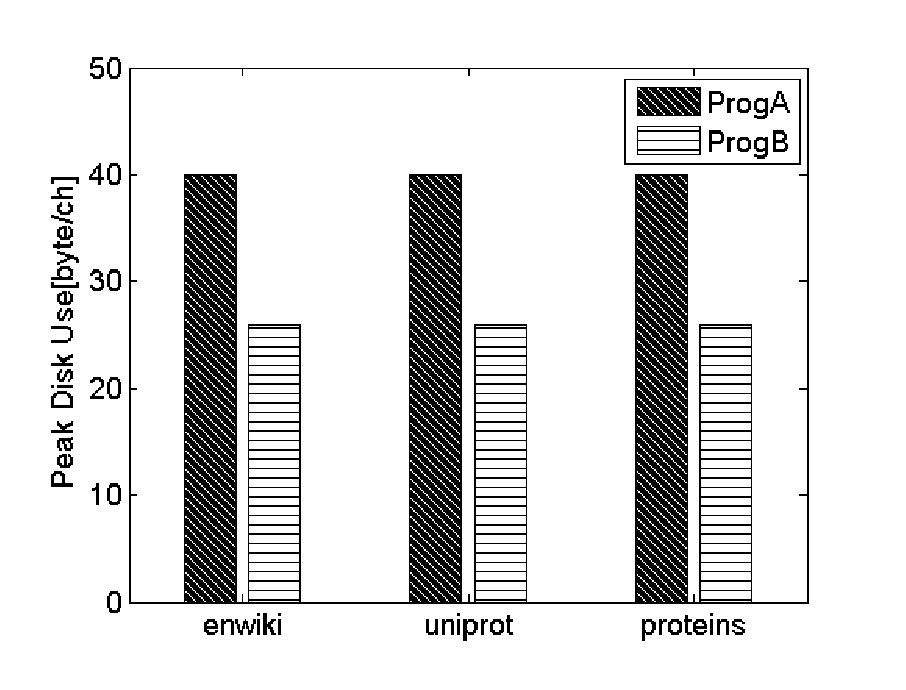
\includegraphics[width = 0.8\columnwidth]{pdu_cmp}
		}
		\hfil
		\subfigure{
			\label{subfig:iov_cmp}
			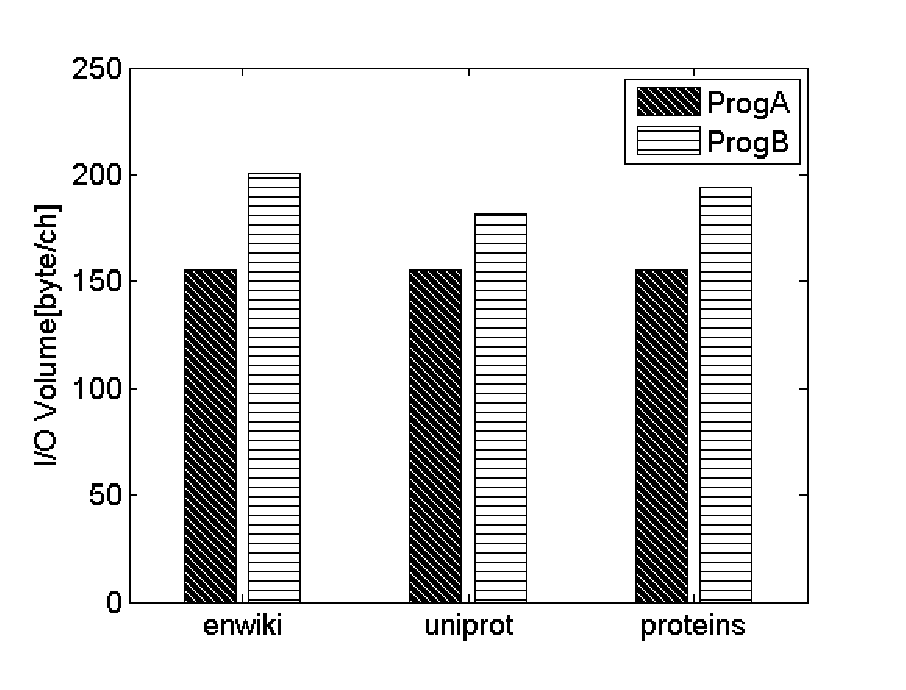
\includegraphics[width = 0.8\columnwidth]{io_cmp}
		}
		\hfil
		\subfigure{
			\label{subfig:ct_cmp}
			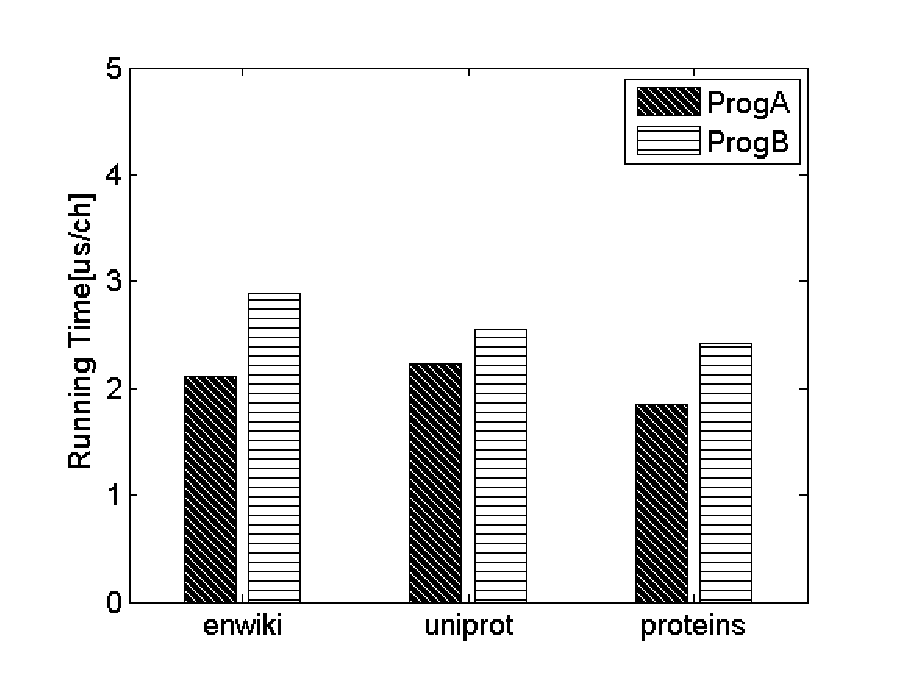
\includegraphics[width = 0.8\columnwidth]{ct_cmp}
		}
		\caption{Experimental results for various corpora.}
		\label{fig:performance_analysis}
	\end{figure}
	
	%figure
	\begin{figure}[htbp!]
		\centering
		\subfigure{
			\label{subfig:pdu_cmp2}
			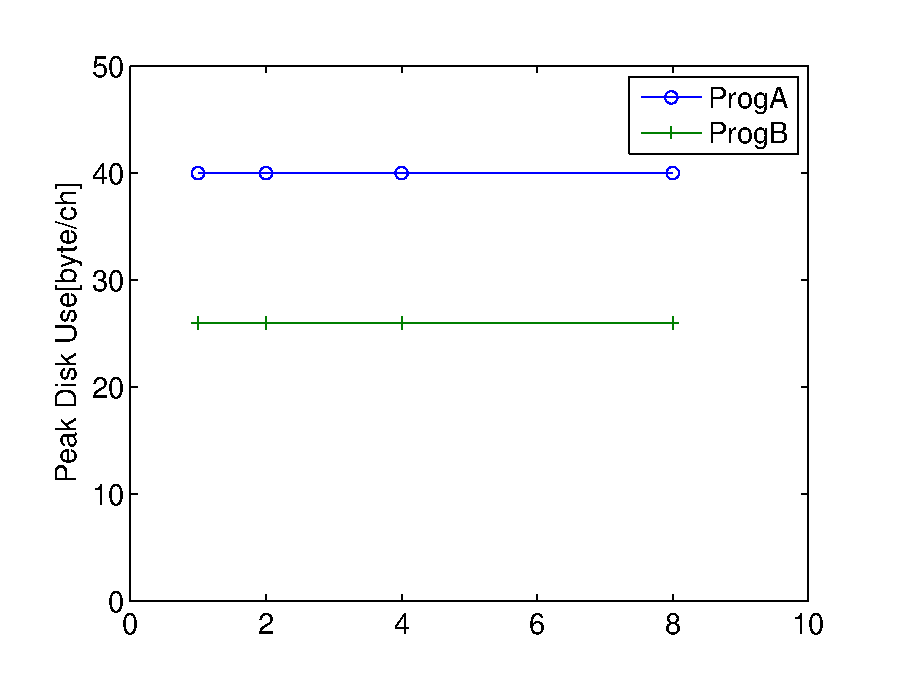
\includegraphics[width = 0.8\columnwidth]{pdu_cmp2}
		}
		\hfil
		\subfigure{
			\label{subfig:iov_cmp2}
			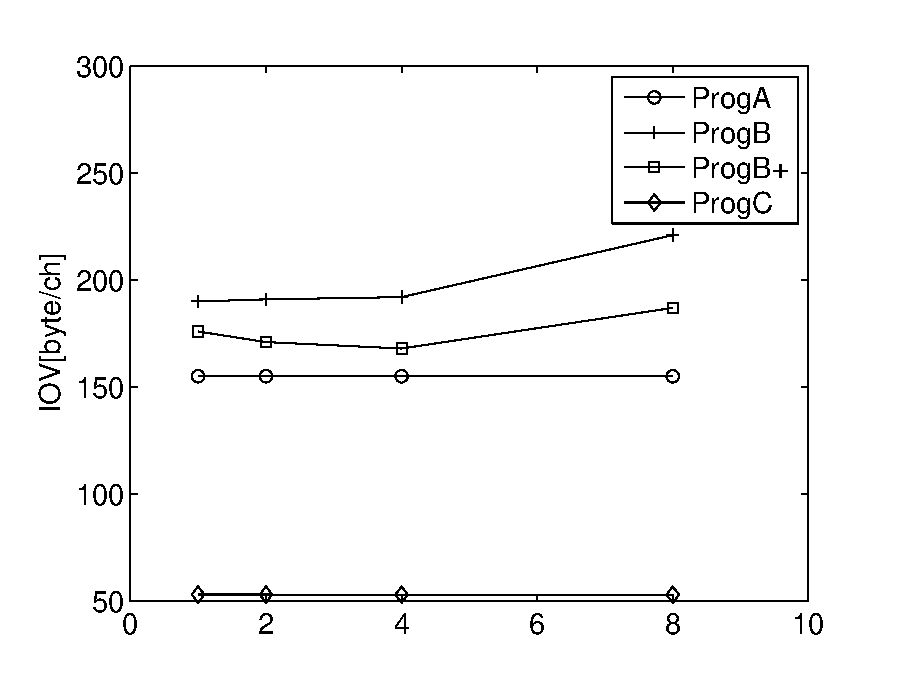
\includegraphics[width = 0.8\columnwidth]{io_cmp2}
		}
		\hfil
		\subfigure{
			\label{subfig:ct_cmp2}
			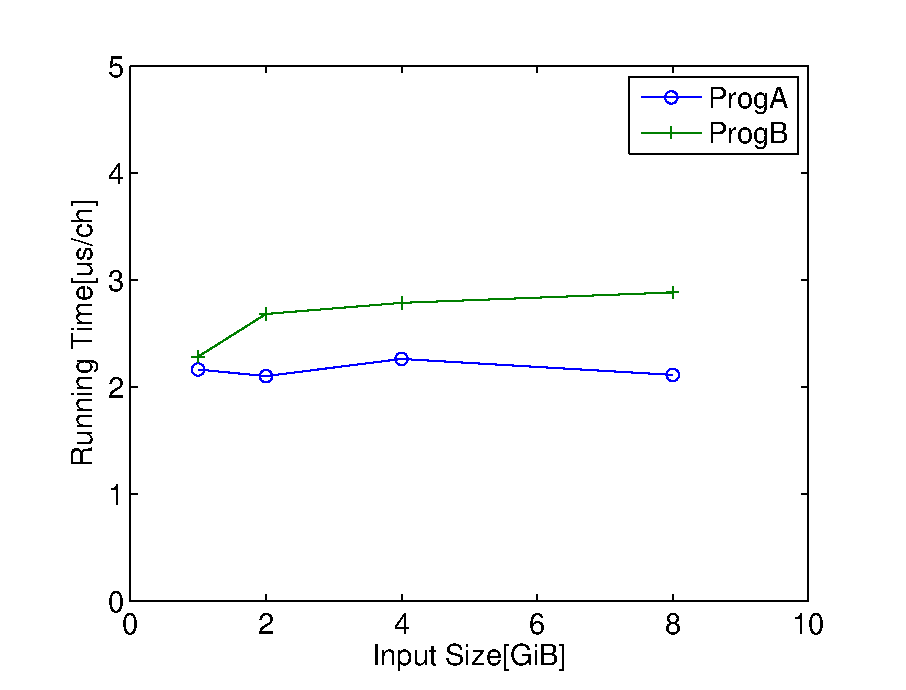
\includegraphics[width = 0.8\columnwidth]{ct_cmp2}
		}
		\caption{Experimental results for prefixes of "enwiki".}
		\label{fig:performance_analysis2}
	\end{figure}
	
	\subsection{Discussions}
	
	It is identified that both programs heavily rely on the performance of the external memory sorter in use. A potential candidate for improving their speed is to adapt a GPU-based multi-way sorter~(e.g.,~\cite{Leischner2010, Davidson2012}) for sorting massive data using external memory. By the aid of these fast sorting algorithms, the throughputs of the programs are expected to nearly approach the I/O bandwidth. Besides, the first two steps of Algorithm~\ref{alg:1} are independent of each other and thus can be executed in parallel for acceleration. This technique can be also applied to check the suffix and LCP arrays of the LMS suffixes in Algorithm~\ref{alg:3}.
	
	Currently, for Algorithm~\ref{alg:3}, step 2 constitutes the space bottleneck. It is worthy of mentioning that this step produces a copy of the suffix and LCP array during the inducing and checking processes. Actually, given that $\Sigma$ is of a constant size and $sa/lcp$ are known already, we can simply scan the input $sa/lcp$ to perform the inducing process and compare each induced suffix/LCP value with that in the given $sa/lcp$ to perform the checking process, resulting in less space consumption. To the end, we must maintain a read pointer for each suffix/LCP bucket in $sa/lcp$ to scan elements in sequence.
	
	\section{Conclusions} \label{sec:conclusion}
	
	We present two probabilistic methods for checking the suffix and LCP arrays in external memory using the Karp-Rabin fingerprinting function. Both methods can be employed to verify the suffix and LCP arrays after their construction, while the second method can be also integrated into an induced-sorting LACA to perform construction and verification in the same time.
	
	We also design the algorithms for these two methods and implement the programs for performance evaluation. An experimental study is conducted to evaluate the time, space and I/O efficiencies.
	The results indicate that the program for the first method outperforms that for the second method in the running time and I/O volume by about 20 percent, while the peak disk use of the latter is about 26/40 = 0.65 as that of the former. There are still quite some opportunities to improve our algorithms and programs for better performance, for this our work has been undergoing.
	
	% Bibliography
	\bibliographystyle{IEEEtran}
	\bibliography{IEEEabrv,bibfile}
	
\end{document}
